\documentclass{article}

% set font encoding for PDFLaTeX, XeLaTeX, or LuaTeX
\usepackage{ifxetex,ifluatex}
\newif\ifxetexorluatex
\ifxetex
  \xetexorluatextrue
\else
  \ifluatex
    \xetexorluatextrue
  \else
    \xetexorluatexfalse
  \fi
\fi

\ifxetexorluatex
  \usepackage{fontspec}
\else
  \usepackage[T1]{fontenc}
  \usepackage[utf8]{inputenc}
  \usepackage{lmodern}
\fi

\usepackage{graphicx}

% used in maketitle
\title{Actividad 7}
\author{Jesús Adrián Zatarain Alvarado}

% Enable SageTeX to run SageMath code right inside this LaTeX file.
% documentation: http://mirrors.ctan.org/macros/latex/contrib/sagetex/sagetexpackage.pdf
% \usepackage{sagetex}

\begin{document}
\maketitle

\section{Introducción}

En la actividad de esta semana se retoma de nuevo el artículo de masas acopladas, se ve la sección tres y parte de la cuarta. En esta ocasión se verán sistemas que no son lineales, se tratará de reproducir los ejemplos mostrados en ambas secciones para poder realizar las gráficas solicitadas

\section{Síntesis}

Este reporte trata sobre las secciones tres y cuatro del artículo. Donde se ven las consecuencias de añadir no linealidad a las ecuaciones anteriormente desarrolladas. Para ello se retoman las ecuaciones y se le hacen ciertos ajustes para que puedan describir a la perfección los siguientes ejemplos a reproducir.
Se añaden a la ecuación coeficientes de no linealidad.

Para el primer ejemplo se introduce a cada variable un valor, que resulta  en que simula ser un oscilamiento periódico por parte de ambos. En el siguiente ejemplo se puede observar que al modificar las variables se ve un comportamiento más definido, y en su esencia, agradable.

Para el ejemplo tres, al modificar los parámetros, se obtiene un movimiento más definido que se nota a primera vista en la gráfica acompañada de este ejemplo.

En el último ejemplo se añaden fuerzas sinoidales a la ecuación. Esto resulta en un movimiento periódico  en su mayor parte.



\section{Desarrollo de la actividad}

\subsection{Ejemplo 3.1}

En esta primera parte se trabaja con ecuaciones no lineales. Con este ejemplo se trata con acoplados descritos por una ecuación de primer grado, no lineal. Se agregó un coeficiente de no linealidad a las ecuaciones anteriores. En esta se ve un movimiento periódico.

\begin{verbatim}

import numpy as np
def vectorfield(w, t, p):
    """
    Defines the differential equations for the coupled spring-mass system.

    Arguments:
        w :  vector of the state variables:
                  w = [x1,y1,x2,y2]
        t :  time
        p :  vector of the parameters:
                  p = [m1,m2,k1,k2,L1,L2,b1,b2]
    """
    x1, y1, x2, y2 = w
    m1, m2, k1, k2, L1, L2, b1, b2, u1, u2, F1, F2, w1, w2 = p

    # Create f = (x1',y1',x2',y2'):
    f = [y1,
         (-b1 * x1 - k1 * x1 -  u1 * x1**3 - k2 * (x1 - x2) + u2 *( x2 - x1)**3 + F1 * np.cos(w1 * t)), 
         y2,
         (-b2 * x2 - k2 * (x2 - x1 ) + u2 * (x2 - x1)**3 +F2 * np.cos(w2 * t))]
    return f
    
\end{verbatim}

En primera instancia, se muestran las gráficas de las fases de los resortes a continuación, donde se nota un movimiento aparentemente peródico.
\begin{center}
  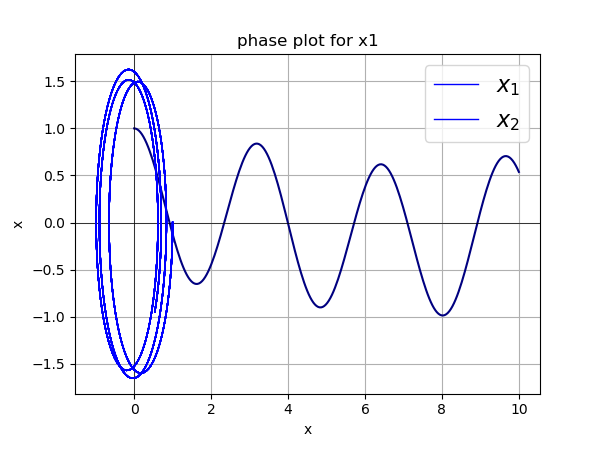
\includegraphics[width=6cm, height=6cm]{ej3_11.png}
\end{center}

\begin{center}
  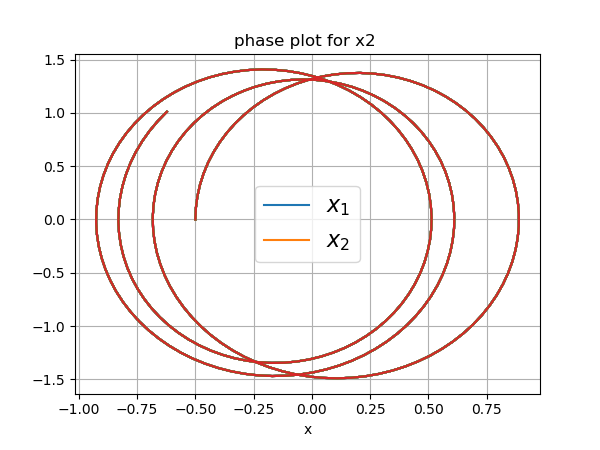
\includegraphics[width=6cm, height=6cm]{ej3_12.png}
\end{center}

Lo siguiente es la elongación de cada uno.

\begin{center}
  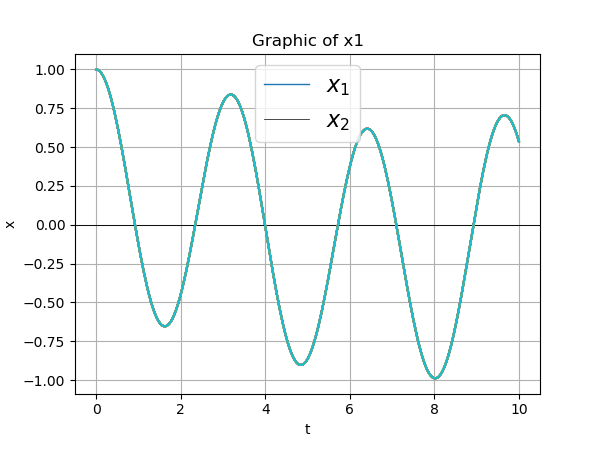
\includegraphics[width=6cm, height=6cm]{ej3_13.png}
\end{center}

\begin{center}
  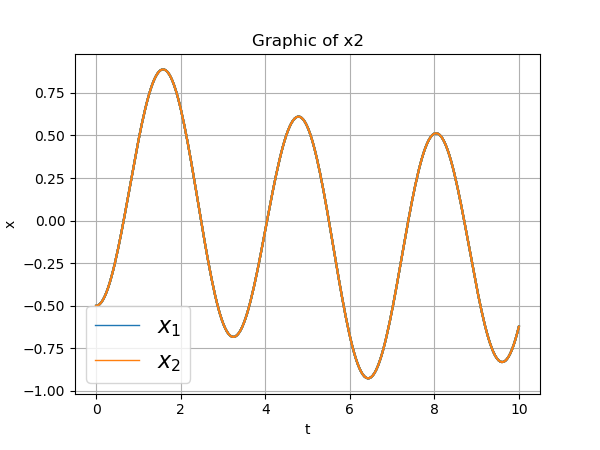
\includegraphics[width=6cm, height=6cm]{ej3_14.png}
\end{center}

Aquí se ve el comportamiento de cada uno
\begin{center}
  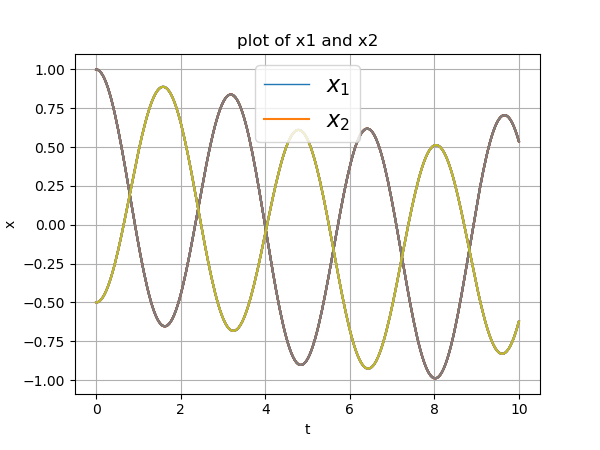
\includegraphics[width=6cm, height=6cm]{ej3_15.png}
\end{center}

En esta gráfica se muestra una comparación directa entre los dos osciladores.
\begin{center}
  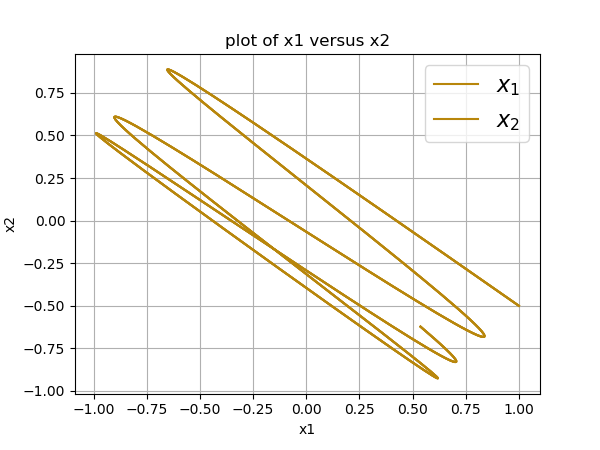
\includegraphics[width=6cm, height=6cm]{ej3_16.png}
\end{center}

\subsection{Ejemplo 3.2}

Para este ejemplo se realizó lo mismo que en el anterior, sólo que se cambiaron ciertos parámetros para notar un cambio.

En las dos gráficas siguientes se puede ver un movimiento más agradable para cada oscilador
\begin{center}
  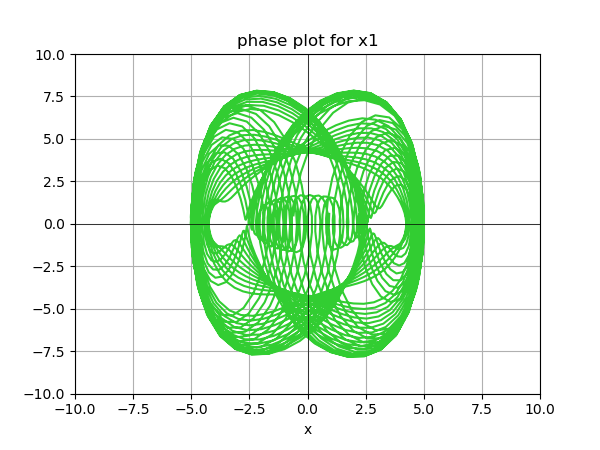
\includegraphics[width=6cm, height=6cm]{ej3_21.png}
\end{center}

\begin{center}
  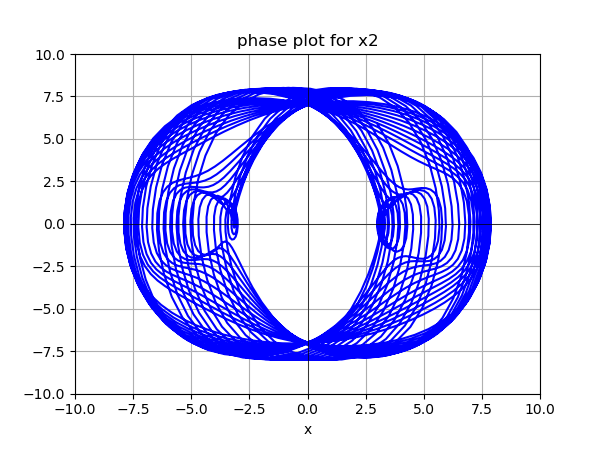
\includegraphics[width=6cm, height=6cm]{ej3_22.png}
\end{center}

Esto es más notorio en la siguiente gráfica donde se comparan los dos
\begin{center}
  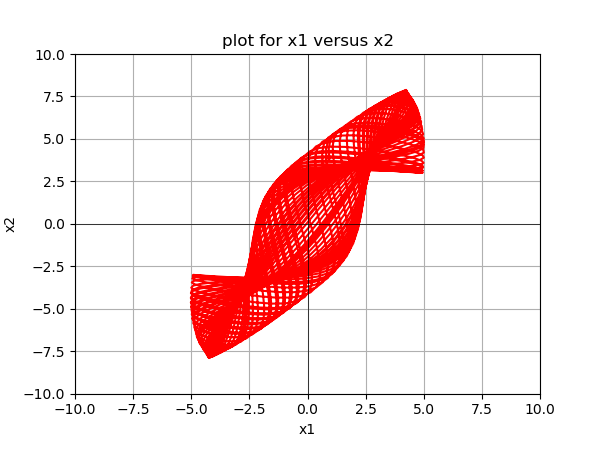
\includegraphics[width=6cm, height=6cm]{ej3_23.png}
\end{center}

\subsection{Ejemplo 3.3}

Para el siguiente ejemplo se trabajó de manera similar para obtener las gráficas. Pero en esta hay un movimiento diferente respecto al anterior ejemplo

\begin{center}
  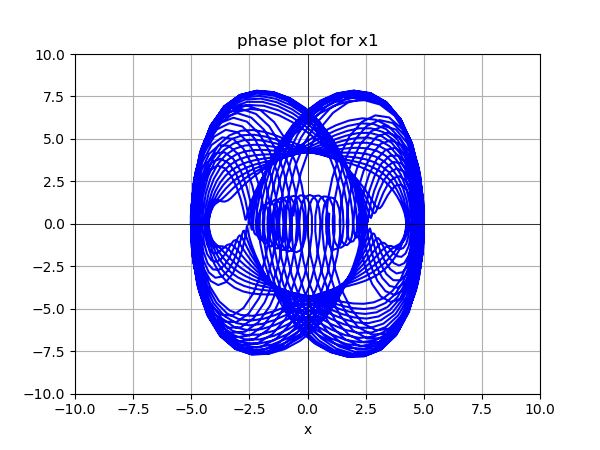
\includegraphics[width=6cm, height=6cm]{ej3_31.png}
\end{center}

\begin{center}
  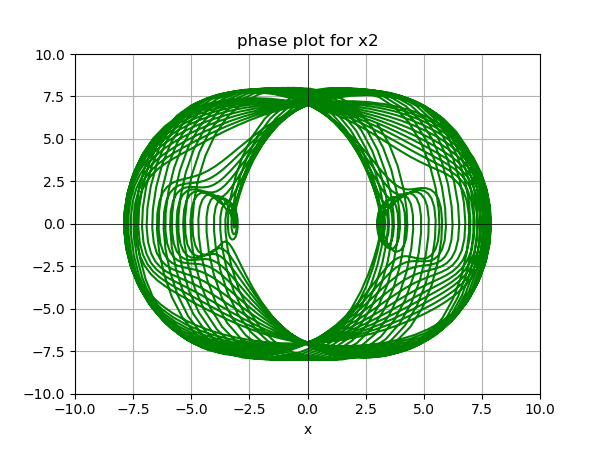
\includegraphics[width=6cm, height=6cm]{ej3_32.png}
\end{center}

\begin{center}
  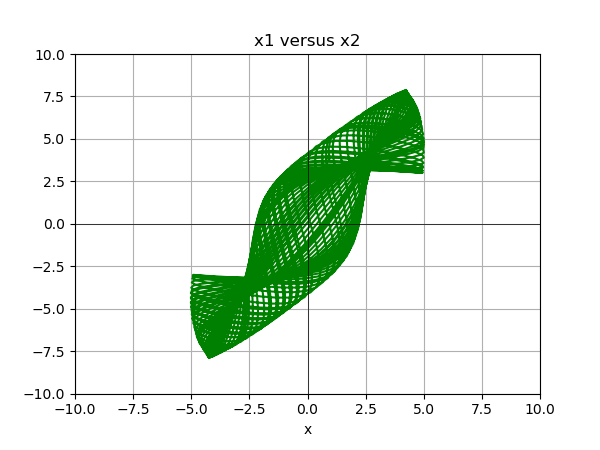
\includegraphics[width=6cm, height=6cm]{ej3_33.png}
\end{center}


\subsection{Ejemplo 4.1}

Para finalizar, en este último ejemplo se añade a las ecuciones fuerzas sinoidales que modifican el movimiento de los osciladores para hacerlos un poco más erráticos.

\begin{verbatim}

import numpy as np
def vectorfield(w, t, p):
    """
    Defines the differential equations for the coupled spring-mass system.

    Arguments:
        w :  vector of the state variables:
                  w = [x1,y1,x2,y2]
        t :  time
        p :  vector of the parameters:
                  p = [m1,m2,k1,k2,L1,L2,b1,b2]
    """
    x1, y1, x2, y2 = w
    m1, m2, k1, k2, b1, b2, u1, u2, w1, w2, F1, F2 = p

    # Create f = (x1',y1',x2',y2'):
    f = [y1,
         (-b1 * y1 - k1 * x1 + u1 * x1**3 - k2 * (x1 - x2) + u2 * (x1 - x2)**3 + F1 * np.cos(w1 * t)) / m1,
         y2,
         (-b2 * y2 - k2 * (x2 - x1) + u2 * (x2 - x1)**3+ F2 * np.cos(w2 * t)) / m2]
    return f
    
\end{verbatim}


En las gráficas también se ve el ciclo límite para cada oscilador y el comportamiento de cada oscilador.
\begin{center}
  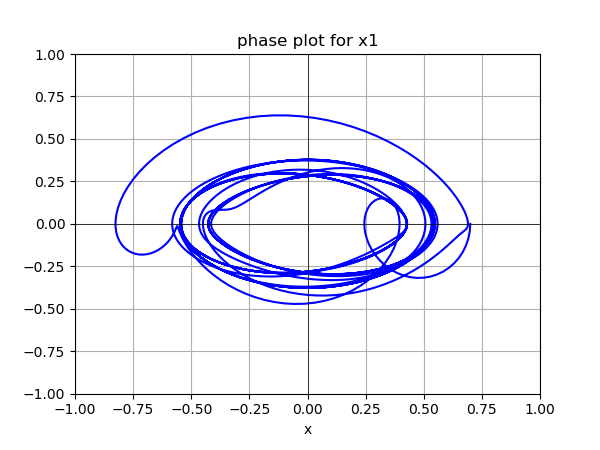
\includegraphics[width=6cm, height=6cm]{ej4_11.png}
\end{center}


\begin{center}
  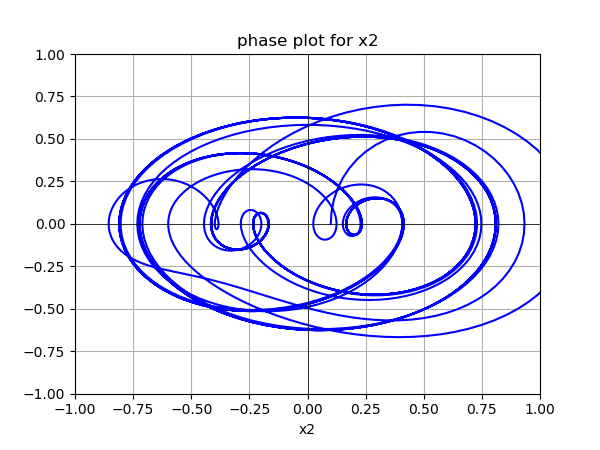
\includegraphics[width=6cm, height=6cm]{ej4_12.png}
\end{center}


\begin{center}
  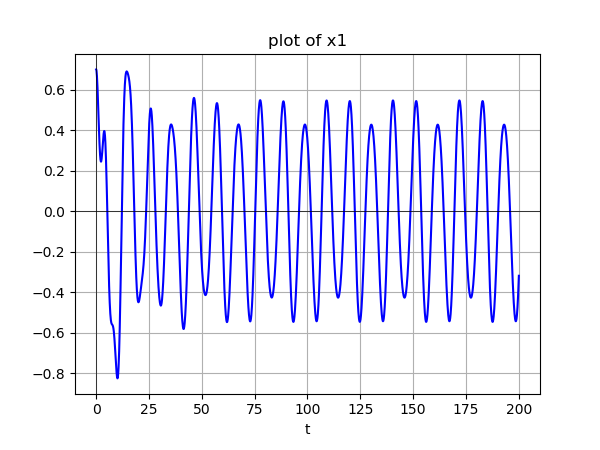
\includegraphics[width=6cm, height=6cm]{ej4_13.png}
\end{center}

\begin{center}
  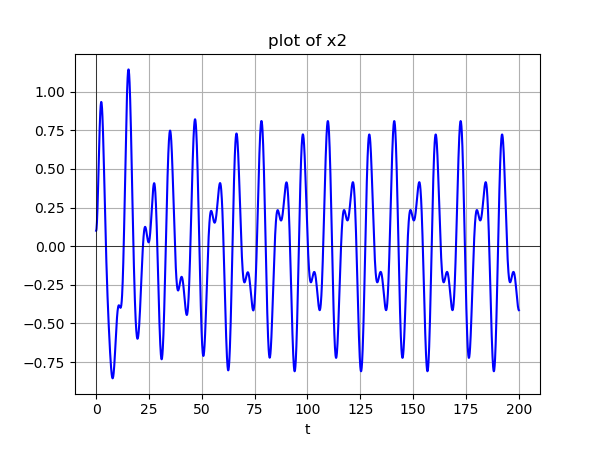
\includegraphics[width=6cm, height=6cm]{ej4_14.png}
\end{center}

\begin{center}
  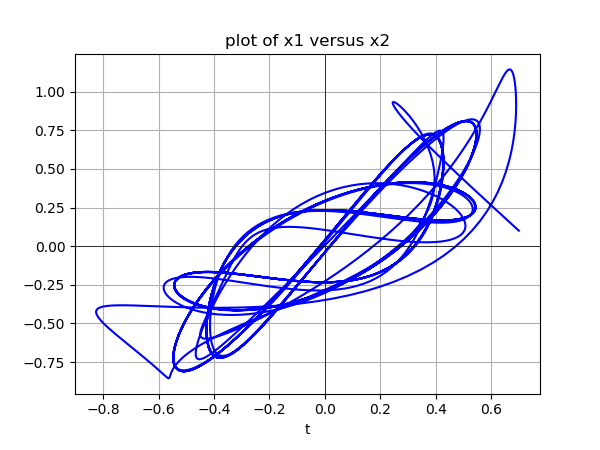
\includegraphics[width=6cm, height=6cm]{ej4_15.png}
\end{center}

\begin{center}
  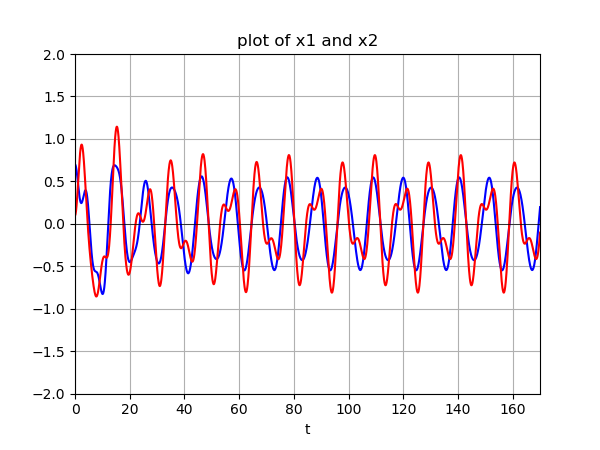
\includegraphics[width=6cm, height=6cm]{ej4_16.png}
\end{center}


\section{Apéndice}

1.- ¿Qué más te llama la atención de la actividad completa? ¿Que se te hizo menos interesante?
\\
\\
Lo más interesante fue ver el comportamiento de los sistemas de masas acopladas no lineales, lo menos interesante fue escribir el código.
\\
\\
2.- ¿De un sistema de masas acopladas como se trabaja en esta actividad, hubieras pensado que abre toda una nueva área de fenómenos no lineales?
\\
\\
Al principio no, pero a medida que iba realizando la actividad, me di cuenta.
\\
\\
3.- ¿Qué propondrías para mejorar esta actividad? ¿Te ha parecido interesante este reto?
\\
\\
Fue interesante la actividad; ver el cómo se pueden describir estos sistemas. Está perfecta la actividad como está.
\\
\\
4.- ¿Quisieras estudiar mas este tipo de fenómenos no lineales?
\\
\\
Sí, fue interesante esta práctica.
\end{document}
